% !TEX program = xelatex
\documentclass[a4paper,14pt,oneside,openany]{memoir}

%%% Задаем поля, отступы и межстрочный интервал %%%

\usepackage[left=30mm, right=15mm, top=20mm, bottom=20mm]{geometry}
\pagestyle{plain}
\parindent=1.25cm
\usepackage{indentfirst}

%%% Задаем языковые параметры и шрифт %%%

\usepackage[english,russian]{babel}
\babelfont[russian]{rm}{Times New Roman}
\babelfont[russian]{tt}{Courier New}

%%% Задаем стиль заголовков и подзаголовков в тексте %%%

\setsecnumdepth{subsection}
\renewcommand*{\chapterheadstart}{}
\renewcommand*{\printchaptername}{}
\renewcommand*{\chapnumfont}{\normalfont\bfseries}
\renewcommand*{\afterchapternum}{\hspace{1em}}
\renewcommand*{\printchaptertitle}{\normalfont\bfseries\centering\MakeUppercase}
\setbeforesecskip{20pt}
\setaftersecskip{20pt}
\setsecheadstyle{\raggedright\normalfont\bfseries}
\setbeforesubsecskip{20pt}
\setaftersubsecskip{20pt}
\setsubsecheadstyle{\raggedright\normalfont\bfseries}

%%% Исправление нумерации секций %%%

\renewcommand{\thesection}{\arabic{section}}
\renewcommand{\thesubsection}{\arabic{subsection}}

%%% Сквозная нумерация рисунков и таблиц %%%

\counterwithout{figure}{chapter}
\counterwithout{table}{chapter}

%%% Выравнивание и переносы %%%

\tolerance 1414
\hbadness 1414
\emergencystretch 1.5em
\clubpenalty=10000
\widowpenalty=10000

%%% Задаем параметры оформления рисунков и таблиц %%%

\usepackage{graphicx}
\usepackage{caption}
\usepackage{subcaption}
\usepackage{float}
\graphicspath{{photo/}}
\captionsetup[figure]{font=small, width=\textwidth, name=Рисунок, justification=centering}
\captiondelim{ --- }
\usepackage[section]{placeins}

%%% Задаем параметры ссылок и гиперссылок %%% 

\usepackage{hyperref}
\hypersetup{
    colorlinks=true,
    linkcolor=red,
    citecolor=red
}

%%% Настраиваем отображение списков %%%

\usepackage{enumitem}
\renewcommand*{\labelitemi}{\normalfont{--}}
\setlist{noitemsep, leftmargin=*}

\begin{document}

% Титульный лист (без номера страницы)
\thispagestyle{empty}

\begin{center}
    МИНИСТЕРСТВО ЦИФРОВОГО РАЗВИТИЯ, СВЯЗИ И МАССОВЫХ \\ КОММУНИКАЦИЙ \\ РОССИЙСКОЙ ФЕДЕРАЦИИ

    \vspace{20pt}

    Федеральное государственное бюджетное образовательное учреждение \\ высшего образования \\
    "Сибирский государственный университет телекоммуникаций и \\ информатики"

    \vspace{20pt}

    Кафедра телекоммуникационных систем и вычислительных средств \\ (ТС и ВС)
\end{center}

\vfill

\begin{center}
    Практическая работа №7 \\
    по дисциплине \\
    \textit{"Web-технологии"}

    \vspace{20pt}

    по теме: \\
    \uppercase{Создание пользователя и отправка электронного письма}
\end{center}

\vfill

\noindent Студент: \\
\textit{Группа ИКС-532 \hfill А.С. Лёшин}

\vspace{20pt}

\noindent Преподаватель: \\
\textit{старший преподаватель \hfill А.В. Андреев}

\vfill

\begin{center}
    Новосибирск 2026 г.
\end{center}

\newpage
\setcounter{page}{2}
\OnehalfSpacing*

\subsection*{Цель работы}
Настроить почтовый сервер на базе iRedMail, обеспечивающий:
\begin{itemize}
    \item Приём и отправку электронных писем через веб-интерфейс Roundcube;
    \item Управление пользователями и доменами через административную панель iRedAdmin;
    \item Проверку работоспособности почтовой системы путём отправки и получения тестового письма.
\end{itemize}

\section{Подготовка инфраструктуры}

Первым этапом настройки является присвоение серверу корректного имени \hyperref[fig:rename]{рисунок \ref*{fig:rename}} и настройка файла. На \hyperref[fig:static_IP]{рисунке \ref*{fig:static_IP}} представлено содержимое данного файла после редактирования.

\begin{figure}[H]
    \centering
    
\includegraphics[width=0.6\textwidth]{photo/photo3.png}
    \caption{Переименование виртуального сервера в mail.leshin.X-532.local}
    \label{fig:rename}
\end{figure}

\begin{figure}[H]
    \centering
    
\includegraphics[width=0.6\textwidth]{photo/photo1.png}
    \caption{Содержимое файла /etc/netplan/00-installer-config.yaml}
    \label{fig:static_IP}
\end{figure}

Проверить можно командой \texttt{ip a}. На \hyperref[fig:ipa]{рисунке \ref*{fig:ipa}} представлен вывод команды.

\begin{figure}[H]
    \centering
    
\includegraphics[width=0.6\textwidth]{photo/photo2.png}
    \caption{Вывод команды ip a}
    \label{fig:ipa}
\end{figure}

\section{Настройка DNS}

Для корректной работы почтового сервера необходимо добавить прямую и обратную записи в DNS на сервере Gateway. На \hyperref[fig:forward]{рисунке \ref*{fig:forward}} показан процесс добавления прямой записи в домен, а на \hyperref[fig:reverse]{рисунке \ref*{fig:reverse}} — обратной записи.

\begin{figure}[H]
    \centering
    
\includegraphics[width=0.8\textwidth]{photo/1.png}
    \caption{Добавление прямой записи в DNS}
    \label{fig:forward}
\end{figure}

\begin{figure}[H]
    \centering
    
\includegraphics[width=0.8\textwidth]{photo/2.png}
    \caption{Добавление обратной записи в DNS}
    \label{fig:reverse}
\end{figure}

\section{Установка iRedMail}

На \hyperref[fig:install_yes]{рисунке \ref*{fig:install_yes}} показано начало установки iRedMail, где необходимо подтвердить начало процесса.

\begin{figure}[H]
    \centering
    
\includegraphics[width=0.6\textwidth]{photo/photo4.png}
    \caption{Запуск установщика iRedMail}
    \label{fig:install_yes}
\end{figure}

Далее выбирается веб-сервер. В данном случае используется Nginx (\hyperref[fig:webserver]{рисунок \ref*{fig:webserver}}).

\begin{figure}[H]
    \centering
    
\includegraphics[width=0.6\textwidth]{photo/photo5.png}
    \caption{Выбор веб-сервера Nginx}
    \label{fig:webserver}
\end{figure}

В качестве базы данных для хранения учётных записей выбирается MariaDB (\hyperref[fig:backend]{рисунок \ref*{fig:backend}}).

\begin{figure}[H]
    \centering
    
\includegraphics[width=0.6\textwidth]{photo/photo6.png}
    \caption{Выбор типа базы данных (MariaDB)}
    \label{fig:backend}
\end{figure}

На \hyperref[fig:domain_ldap]{рисунке \ref*{fig:domain_ldap}} указано имя домена для LDAP. В данном случае используется структура \texttt{dc=leshin,dc=X-532,dc=local}.

\begin{figure}[H]
    \centering
    
\includegraphics[width=0.8\textwidth]{photo/photo8.png}
    \caption{Указание имени домена}
    \label{fig:domain_ldap}
\end{figure}

Далее задаётся пароль администратора базы данных (\hyperref[fig:mysql_pass]{рисунок \ref*{fig:mysql_pass}}).

\begin{figure}[H]
    \centering
    
\includegraphics[width=0.8\textwidth]{photo/photo9.png}
    \caption{Установка пароля MySQL root}
    \label{fig:mysql_pass}
\end{figure}

На \hyperref[fig:admin_mail]{рисунке \ref*{fig:admin_mail}} вводится email администратора почтовой системы.

\begin{figure}[H]
    \centering
    
\includegraphics[width=0.8\textwidth]{photo/photo10.png}
    \caption{Указание email администратора}
    \label{fig:admin_mail}
\end{figure}

Затем задаётся пароль для администратора почты (\hyperref[fig:admin_pass]{рисунок \ref*{fig:admin_pass}}).

\begin{figure}[H]
    \centering
    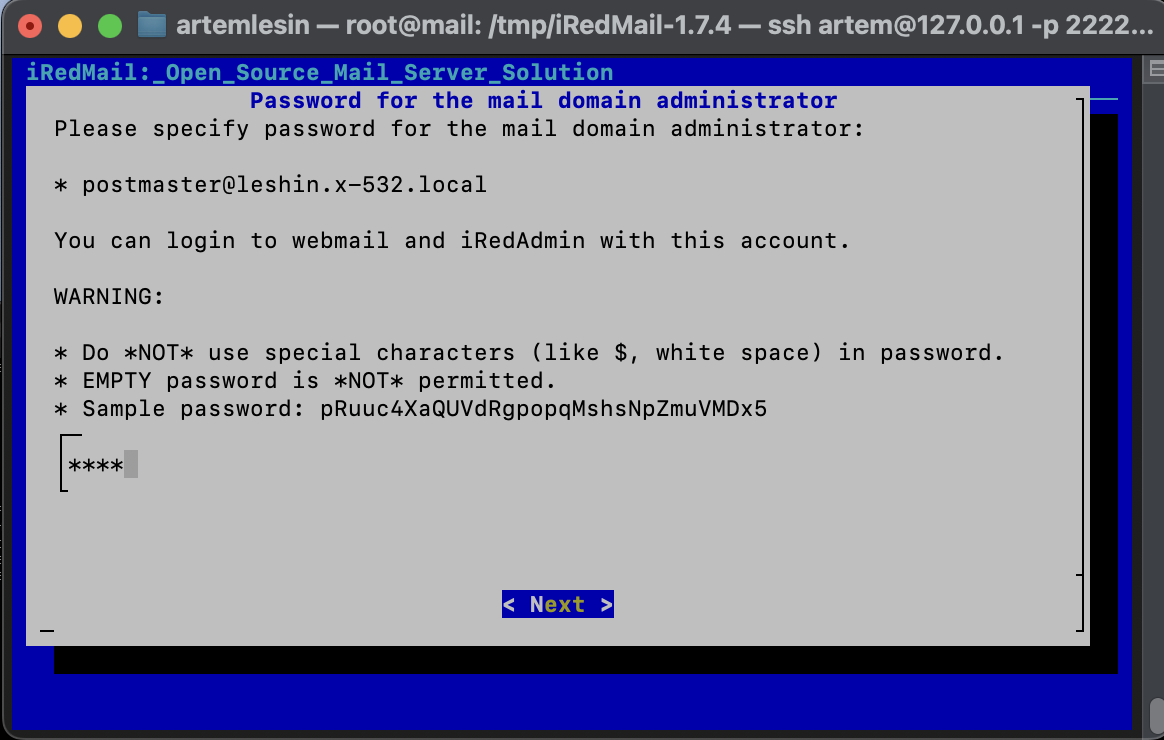
\includegraphics[width=0.8\textwidth]{photo/photo11.png}
    \caption{Установка пароля почтового администратора}
    \label{fig:admin_pass}
\end{figure}

На этапе выбора дополнительных компонентов (\hyperref[fig:components]{рисунок \ref*{fig:components}}) выбирается веб-почта Roundcube.

\begin{figure}[H]
    \centering
    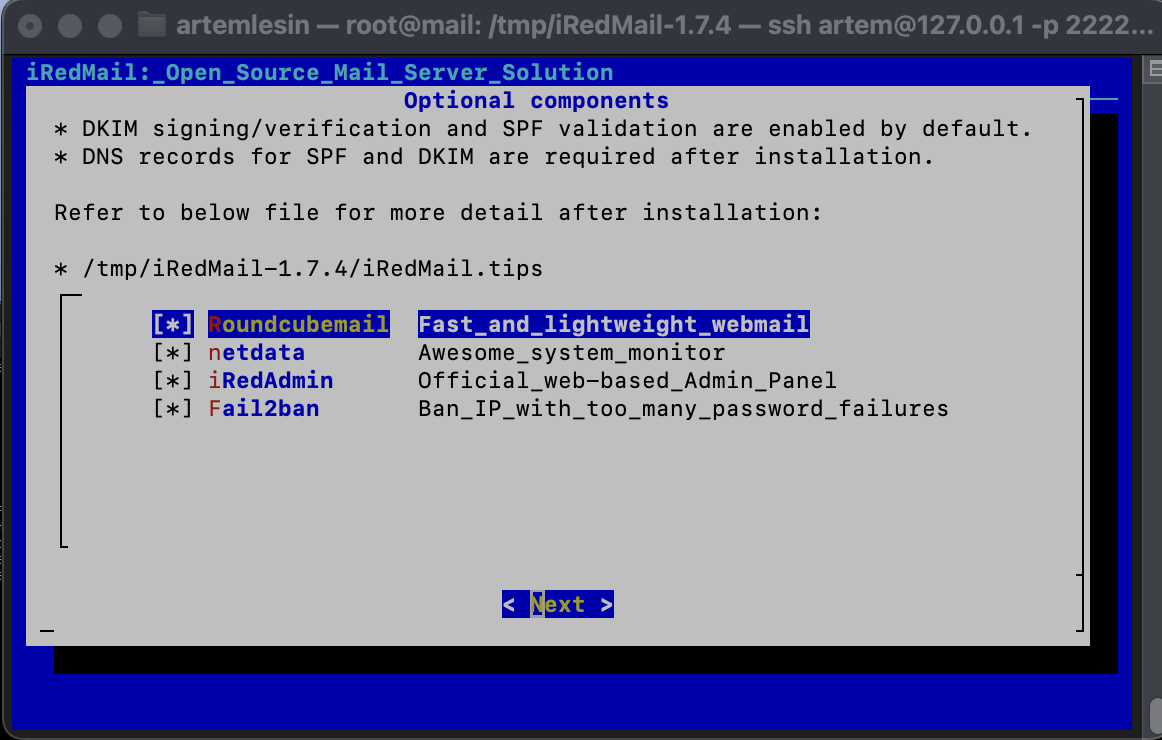
\includegraphics[width=0.8\textwidth]{photo/photo12.png}
    \caption{Выбор компонентов почтовой системы}
    \label{fig:components}
\end{figure}

После завершения установки сервер перезагружается.

\section{Управление почтовым сервером}

После перезагрузки необходимо перейти по адресу \\
\texttt{https://mail.leshin.X-532.local/iredadmin} \\
для входа в панель администратора (\hyperref[fig:login_page]{рисунок \ref*{fig:login_page}}).

\begin{figure}[H]
    \centering
    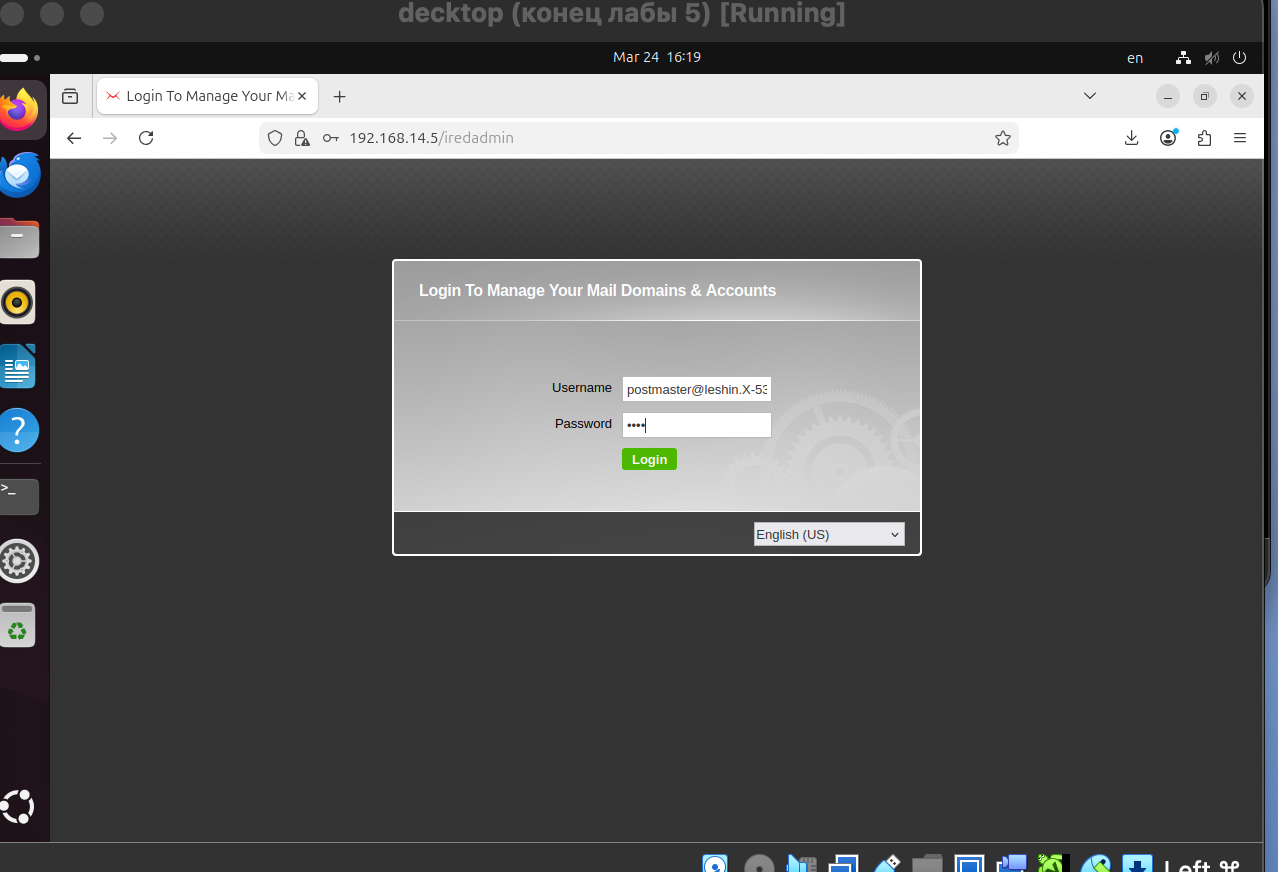
\includegraphics[width=0.8\textwidth]{photo/photo13.png}
    \caption{Страница входа в iRedAdmin}
    \label{fig:login_page}
\end{figure}

Успешный вход в панель управления показан на \hyperref[fig:admin_panel]{рисунке \ref*{fig:admin_panel}}.

\begin{figure}[H]
    \centering
    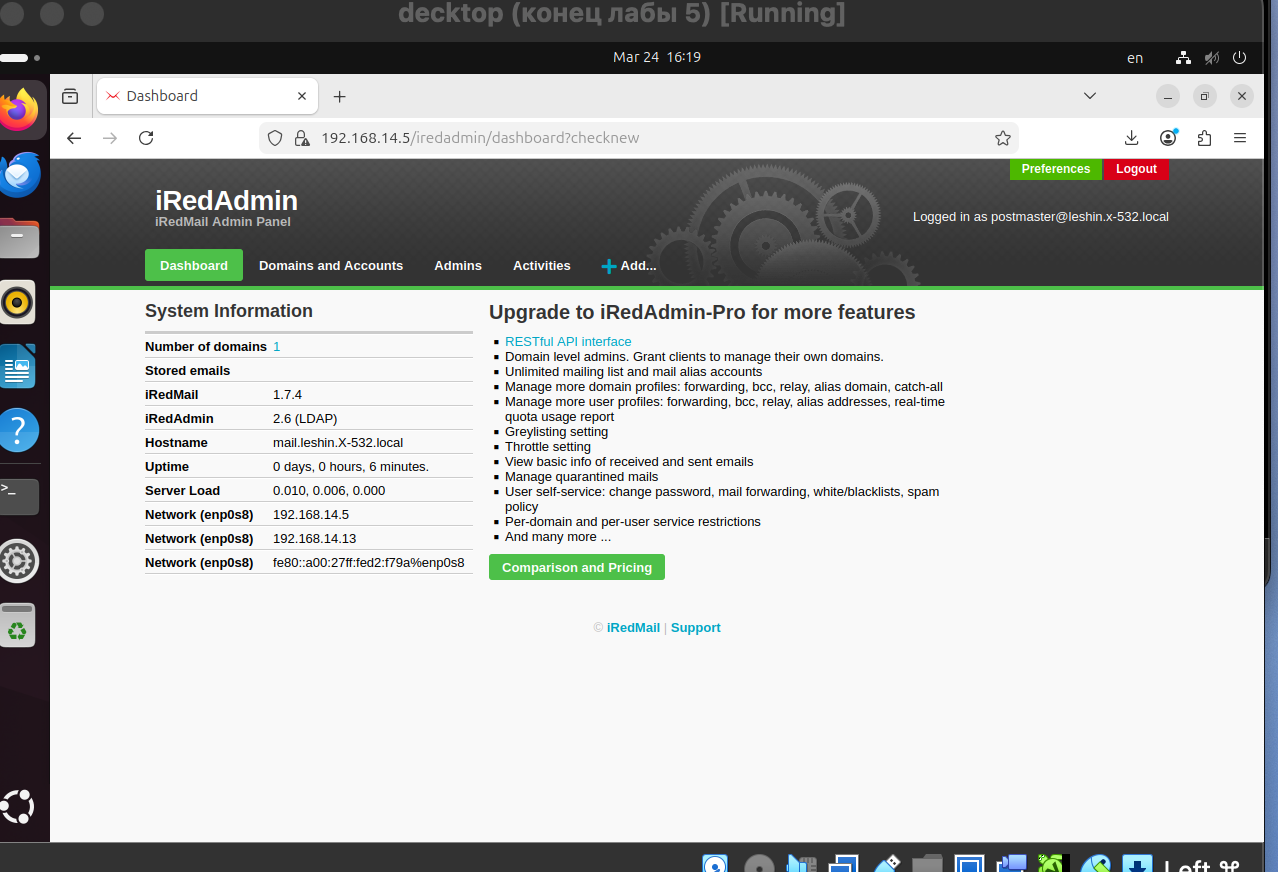
\includegraphics[width=0.8\textwidth]{photo/photo14.png}
    \caption{Интерфейс iRedAdmin после входа}
    \label{fig:admin_panel}
\end{figure}

В панели администратора создаётся новый почтовый ящик (\hyperref[fig:create_user]{рисунок \ref*{fig:create_user}}).

\begin{figure}[H]
    \centering
    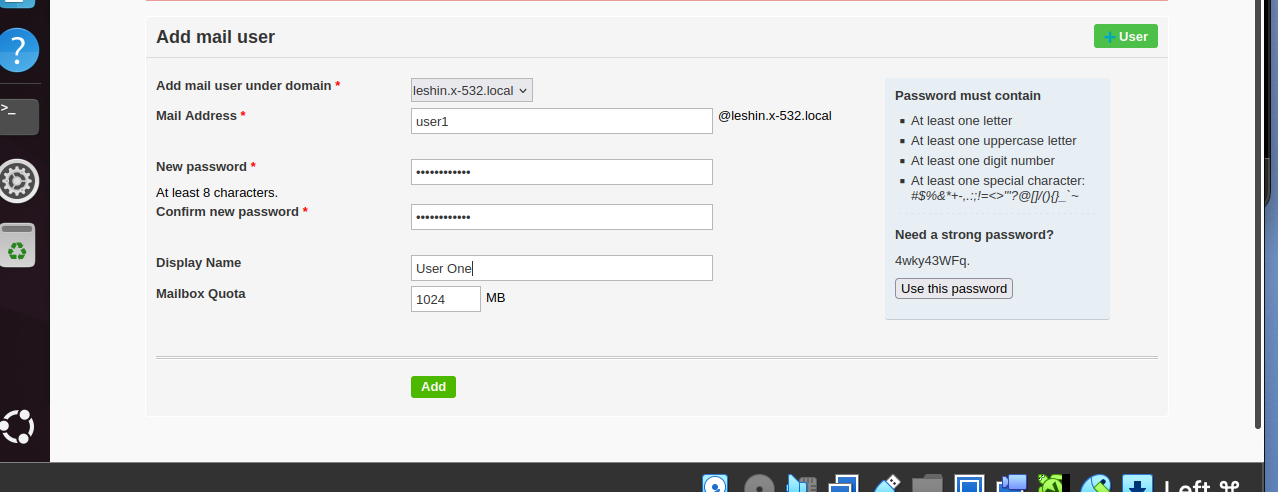
\includegraphics[width=0.8\textwidth]{photo/photo15.png}
    \caption{Создание нового пользователя}
    \label{fig:create_user}
\end{figure}

Для проверки работоспособности необходимо войти в веб-почту по адресу \texttt{https://mail.leshin.X-532.local/mail} под учётной записью \texttt{user1@leshin.X-532.local} (\hyperref[fig:webmail_login]{рисунок \ref*{fig:webmail_login}}).

\begin{figure}[H]
    \centering
    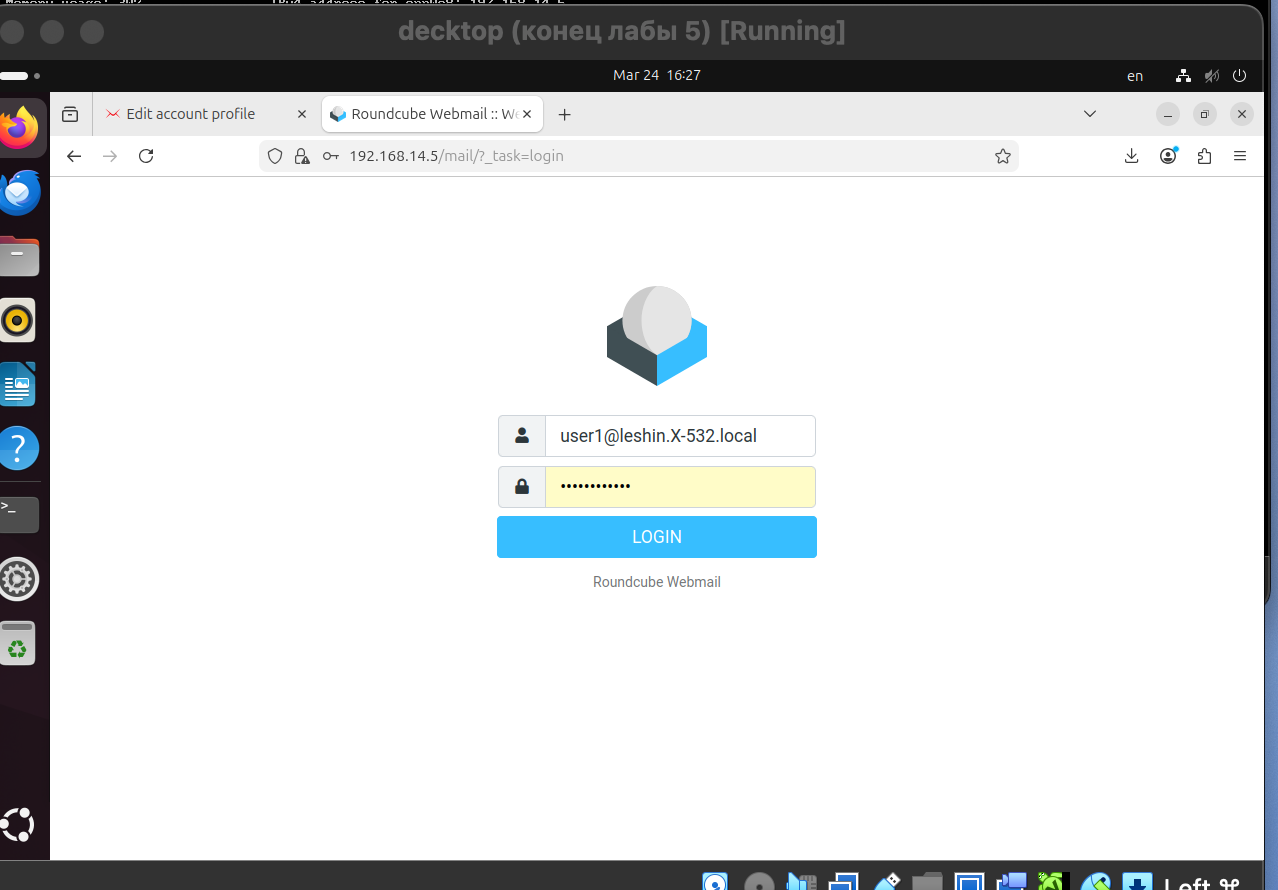
\includegraphics[width=0.8\textwidth]{photo/photo16.png}
    \caption{Вход в веб-почту Roundcube}
    \label{fig:webmail_login}
\end{figure}

В интерфейсе Roundcube создаётся тестовое письмо (\hyperref[fig:write_email]{рисунок \ref*{fig:write_email}}).

\begin{figure}[H]
    \centering
    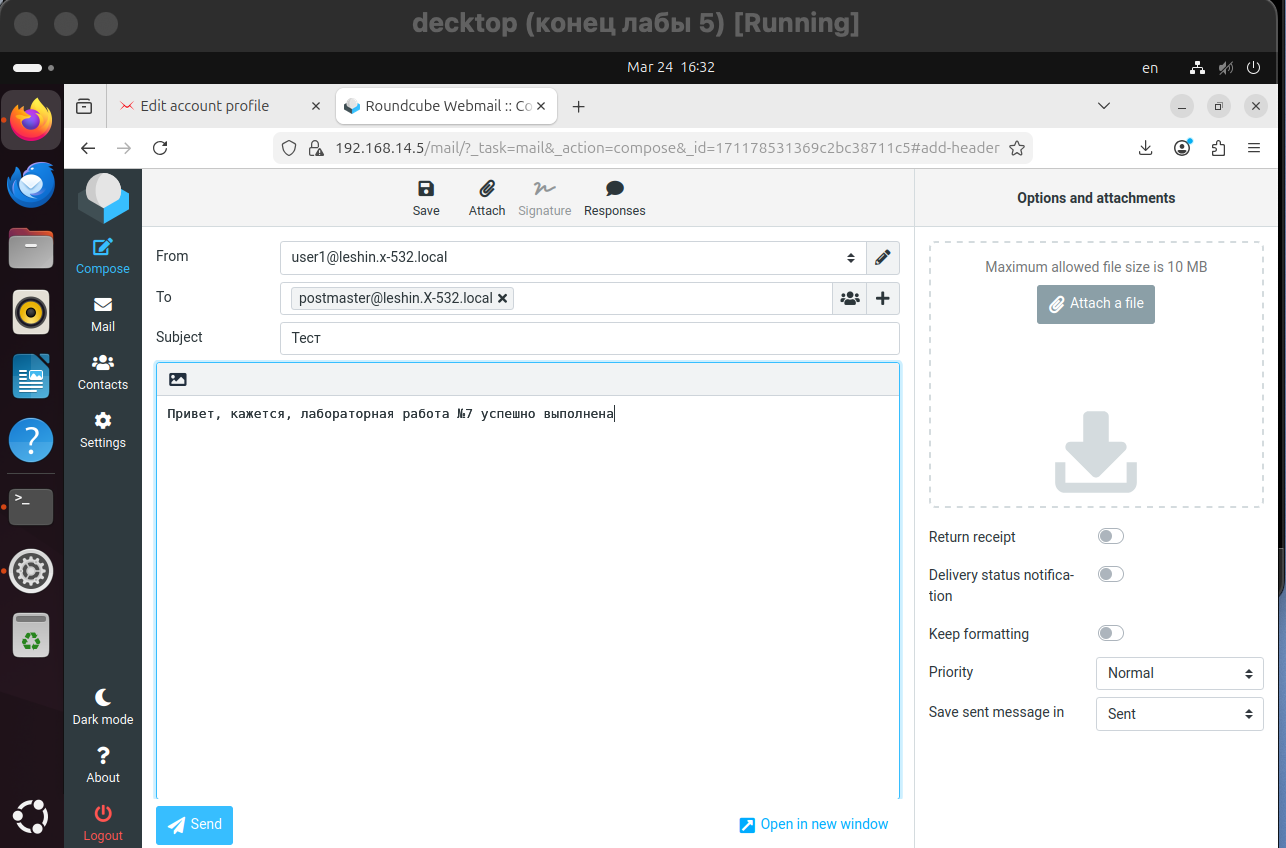
\includegraphics[width=0.8\textwidth]{photo/photo17.png}
    \caption{Создание тестового письма}
    \label{fig:write_email}
\end{figure}

На \hyperref[fig:email_received]{рисунке \ref*{fig:email_received}} видно, что письмо успешно доставлено адресату.

\begin{figure}[H]
    \centering
    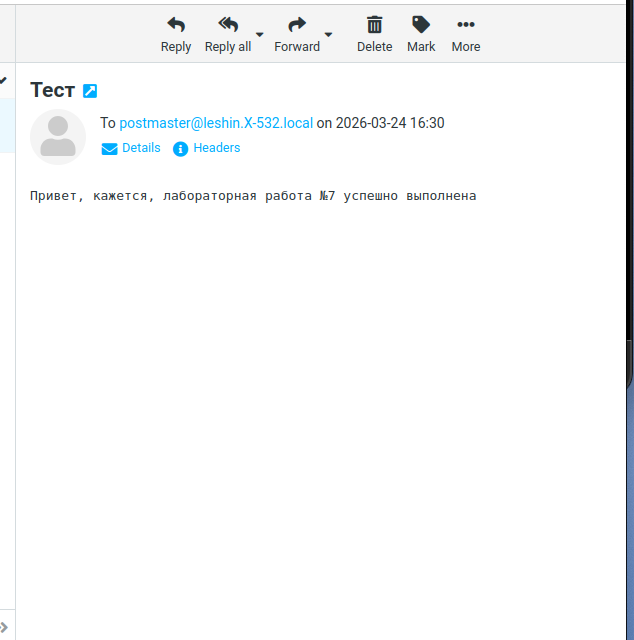
\includegraphics[width=0.8\textwidth]{photo/photo18.png}
    \caption{Полученное письмо в ящике}
    \label{fig:email_received}
\end{figure}

\section*{Заключение}
\addcontentsline{toc}{section}{Заключение}

В ходе выполнения работы был успешно развёрнут почтовый сервер на базе iRedMail. Выполнены следующие задачи:
\begin{enumerate}
    \item Подготовлена инфраструктура — создана ВМ mail;
    \item Настроены DNS-записи для почтового сервера;
    \item Установлен и настроен iRedMail;
    \item Создана учётная запись \texttt{user1@leshin.X-532.local};
    \item Проверена работоспособность — отправлено и получено тестовое письмо через веб-интерфейс Roundcube.
\end{enumerate}

\end{document}